%===============================
%------------------------------
\section{Information and Bits}
%------------------------------
%===============================

%Information as defined by Claude Shannon is a statistical concept. Alternatives

%---------------------------------------------
\subsection{Probability}
%---------------------------------------------

We will set up and formalize notations to talk about randomness using the context of statistical experiments. These can be actual (``artificial") experiments in the lab, or natural processes, the outcomes of which are random.

Denote by $\Omega$ the set of all possible outcomes ({\bf events}) of a statistical experiment, usually called the {\bf sample space} or the ``universe".

%Let $\Omega$ be the set of all possible outcomes of a statistical experiment, also known as the {\bf sample space} or the ``universe".

\begin{example}[\bf Coin toss]\leavevmode
	The sample space consists of the outcome that the coin comes up head (H) or tail (T): $\Omega = \{H,T\}$.
\end{example} 
\begin{example}[\bf Die roll]\leavevmode
	The sample space is the number on the face of a die: $\Omega = \{1,2,3,4,5,6\}$.
\end{example}
\begin{margintable}
	\begin{tabular}{ |c|c|c| } 
		\hline
		& \multicolumn{1}{|p{1cm}|}{\centering \scriptsize{Logical} \\ \scriptsize{operation}} & \multicolumn{1}{|p{1cm}|}{\centering \scriptsize{Set} \\ \scriptsize{operation}}  \\
		\hline 
		NOT & $\neg A$ & $\overline{A}$ \\ 
		AND & $A \wedge B$ & $A \cap B$ \\
		OR & $A \vee B$ & $A \cup B$	\\
		\hline
	\end{tabular}
	\caption{Symbols for elementary logical operations and the corresponding set operations, which we use interchangeably.}
	\label{table:logical_operations}
\end{margintable}
Each outcome of a statistical experiment can be associated with a {\bf logical proposition} in the obvious way. For example, the result ``1" of a die roll is associated with the proposition ``the die is rolled and we obtained a 1". Every such proposition can be assigned a binary value TRUE or FALSE. 
These outcomes do not exhaust all possible events because we can combine events using logical (Boolean) operations such as AND or OR to create new logical propositions.


An {\bf empty event} (set) is denoted by $\emptyset$. Self-evidently,
\begin{align}
	A \wedge \overline{A} = \emptyset, && A \vee \overline{A} = \Omega.
\end{align}

Whenever $\Omega$ is a finite set, we can always find an elementary set of disjoint ({\bf mutually exclusive}) propositions called {\bf elementary events} or {\bf atomic events} $\{E_j\}_j$: %(These are nothing but the outcomes of our statistical experiment.) 
\begin{align}
	E_j \wedge E_k = \begin{cases}
		E_j, & j=k, \\
		\emptyset, & j\neq k.
	\end{cases}
\end{align}
The set of all possible events i.e. logical combinations of all atomic events, constitutes a \emph{Boolean algebra} $\{0,1\}^n$ whose size is $2^n$ if there are $n$ atomic events.
It is the set $\{0,1\}^n$ because an event is defined by whether each atomic event is absent or present in the Boolean formula $E_{j_1} \vee E_{j_2} \vee \cdots \vee E_{j_m}$, $m \le n$.
\begin{marginfigure}
	\centering
	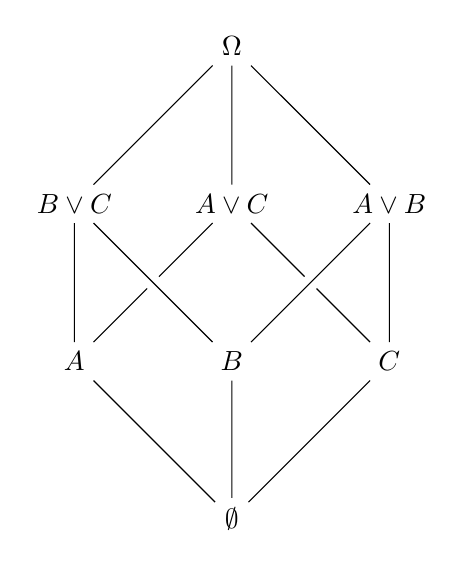
\begin{tikzpicture}
		\node (max) at (0,4) {$\Omega$};
		\node (a) at (-2,2) {$B\vee C$};
		\node (b) at (0,2) {$A\vee C$};
		\node (c) at (2,2) {$A\vee B$};
		\node (d) at (-2,0) {$A$};
		\node (e) at (0,0) {$B$};
		\node (f) at (2,0) {$C$};
		\node (min) at (0,-2) {$\emptyset$};
		\draw (min) -- (d) -- (a) -- (max) -- (b) -- (f)
		(e) -- (min) -- (f) -- (c) -- (max)
		(d) -- (b);
		\draw[preaction={draw=white, -,line width=6pt}] (a) -- (e) -- (c);
	\end{tikzpicture}
	\label{}
	\caption{The Hesse diagram of a Boolean algebra with three atomic events $A, B$, and $C$. Going up in the diagram corresponds to the logical operation OR ($\vee$), while going down corresponds to AND ($\wedge$).}
\end{marginfigure}

\begin{mybox}
	 $\{0,1\}^n$ is also the \emph{power set} $\mathcal{P}(\Omega)$, the set of all subsets of $\Omega$.
	The power set $X^Y$ is the set of all functions from $Y$ to $X$. There are exactly $|X|^{|Y|}$ such functions, hence the notation. (Why? For each input in $Y$, one can choose an output from all possible choices of $x\in X$.)
\end{mybox}

So far we have not yet talked about assigning probabilities to events. There is a long-standing debate about what a probability actually means, but for us a probability is just a number between 0 (the event never occurs) and 1 (the event occurs with certainty).

\begin{definition}[\bf Probability axioms]\leavevmode
	
	\begin{enumerate}
		\item $\Pr(A) \ge 0$,
		\item $\Pr(A) =1 \iff A$ is certain,
		\item $\Pr(A\vee B) = \Pr(A)+\Pr(B)$ if $A\wedge B  =\emptyset$
	\end{enumerate}
\end{definition}
These axioms are sufficient to derive any other identities such as 
\begin{align}
	\Pr(\neg A) &= 1-\Pr(A), \\
	\Pr(A\vee B) &= \Pr(A) + \Pr(B) - \Pr(A\wedge B).
\end{align}

Let us formalize one more thing: a {\bf random variable} $X$ is a variable that takes a value $x\in \Omega$ with probability $\Pr(X=x)$. We usually write $X\sim f$ to mean that values of $X$ are distributed according to a probability distribution $f$.
\begin{align*}
	\boxed{\textrm{Random variable} \leftrightarrow \textrm{Statistical experiment}}
\end{align*}
We will use interchangeably the notations 
\begin{align}
	\Pr(X=x) \equiv p_X(x) \equiv p(x).
\end{align}
\begin{definition}[\bf $k$th moment]\leavevmode
	\begin{align}
		{\color{magenta}\underbracket{\color{black}\E[X^k]}_{\mathclap{\substack{\textrm{Mathema-} \\ \textrm{ticians'} \\ \textrm{notation}}}}} \equiv {\color{teal}\underbracket{\color{black}\av{X^k}}_{\mathclap{\substack{\textrm{Physicists'} \\ \textrm{notation}}}}}
		\equiv \av{x^k} = \sum_x x^k p(x)
	\end{align}
\end{definition}
\noindent The {\bf mean value}, also known as the average or the expectation value, is the first moment, whereas
the {\bf variance} is the part of the second moment that is independent of the first moment.\mn{The variance is the second \href{https://en.wikipedia.org/wiki/Cumulant}{cumulant}. The Gaussian distribution is the unique probability distribution whose cumulants all vanish except the first and the second.} 
\begin{align}
	\textrm{Var}(X) \equiv \sigma_x^2 = \av{(X-\av{X})}^2 = \av{X^2} - \av{X}^2
\end{align}

\begin{example}[\bf Bernoulli trials]\leavevmode
	
	Suppose that $X$ takes values $n$, the number of heads obtained in $N$ independent tosses of a coin with a bias $p$. (More about independence later.) The probability of such an event is given by the \emph{binomial distribution} $X\sim B(N,p)$. 
	
	\begin{align}
	\left(\parbox{8em}{\centering Probability of obtaining a particular sequence with exactly $n$ heads}\right) &= p^n(1-p)^{N-n} \\
	\Pr(X=n)  = \left(\parbox{8em}{\centering Probability of obtaining \emph{any} particular sequence with exactly $n$ heads}\right) &= {N \choose n}p^n(1-p)^{N-n}
	\end{align}

	The normalization can be verified directly. Let $q=1-p$.
	\begin{align}
		\sum_{n=0}^N \Pr(X=n) = \sum_{n=0}^N{N \choose n}p^n q^{N-n} 
		= (p+q)^N = 1,
	\end{align}
	where we have used the binomial theorem in the second-to-last equality.
	\begin{align}
		\av{n} &= \sum_{n=0}^N np(n) = \sum_{n=0}^N n{N \choose n}p^n q^{N-n} \\
		&= p \pdv{p}\sum_{n=0}^N {N \choose n}p^n q^{N-n}
		= p \pdv{p}(p+q)^N \\
		&= Np \cancelto{1}{(p+q)^{N-1}} = Np
	\end{align}
	The same trick can be used to calculate the variance  $\sigma^2 = Np(1-p)$.
\end{example}


%---------------------------------------------
%\subsection{Correlation}
%---------------------------------------------

Things become interesting when there are two or more random variables.
\begin{definition}[\bf Joint probability]\leavevmode
	\begin{align}
		\Pr(X=x,Y=y) \equiv p_{XY}(x,y) \equiv p(x,y)
	\end{align} 
	is the probability that both the outcomes $x$ and $y$ happen.
\end{definition}

\begin{definition}[\bf Marginal probability]\leavevmode
	\mnf{\begin{align}
			p(x) = {\color{maincolor}\underbracket{\color{black}p(x,y)}_{\mathclap{\substack{ \textrm{Probability} \\ \textrm{that both $x$} \\ \textrm{and $y$ occur} }}} } 
			\; + \; {\color{eqcolor}\underbracket{\color{black}p(x,\neg y)}_{\mathclap{\substack{\textrm{Probability} \\ \textrm{that $x$ occurs} \\ \textrm{but $y$ doesn't} }}} }
	\end{align}} 
	\begin{align}
		p(x) = \sum_y p(x,y), && p(y) = \sum_x p(x,y),
	\end{align}
\end{definition}
\noindent A marginal probability is the probability that an outcome described by one of the random variables may occur without looking at the outcome of the other random variable.

\begin{definition}[\bf Conditional probability]\leavevmode
		
	For $\Pr(Y=y) \neq 0$,
	\begin{align}
		\Pr(\smash{X=x|\underbracket{Y=y}_{\textrm{Condition}}}) \equiv p(x|y) = \frac{p(x,y)}{p(y)}
	\end{align}
	is the probability that the event $x$ occurs \emph{if} the event $y$ also occurs.
\end{definition}
\noindent A conditional probability distribution for a fixed value of $Y$ must normalize to 1.
\begin{align}
	\sum_x p(x|y) = \frac{1}{p(y)} \sum_x p(x,y) = \frac{\cancel{p(y)}}{\cancel{p(y)}} = 1
\end{align}
Other useful equalities are obtained from these basic definitions.
\begin{lemma}[\bf Law of total probability]\leavevmode
	\begin{align}
		p(x) = \sum_y p(x|y)p(y)
	\end{align}
\end{lemma}

\begin{lemma}[\bf Bayes' theorem]\leavevmode
	\begin{align}
		p(x|y) = \frac{p(y|x)p(x)}{p(y)}.
	\end{align}
\end{lemma}
\noindent Bayes' theorem emphasizes that $p(x|y)$ and $p(y|x)$ are not equal in general. As an example, the probability of having Covid given a positive test result is not equivalent to the probability of testing positive when actually having Covid.
Usually when computing $p(x|y)$ via Bayes' theorem, one computes the denominator $p(y)$ using the law of total probability.

\begin{definition}
	Events $x$ and $y$ are {\bf independent} if 
	\begin{align}
		p(x,y) = p(x)p(y).
	\end{align}
	Otherwise, they are {\bf correlated}. We also say that two random variables $X$ and $Y$ are correlated if $p(x,y) \neq p(x)p(y)$ for some $x$ and $y$.
\end{definition}
\noindent In words, events $x$ and $y$ are independent if looking at the outcome of one of them does not give you any information about the other event i.e. does not make the other event more or less likely to occur.
\begin{align}
	p(x|y) = \frac{p(x,y)}{p(y)} = \frac{p(x)\cancel{p(y)}}{\cancel{p(y)}} = p(x).
\end{align}

\begin{mybox}
Mutually exclusive events cannot be independent. If I flip a coin and it comes up head, it could not have come up tail. Mathematically, this is because, if $x\wedge y =\emptyset$, then $p(x,y)=0$ but $p(x)p(y)$ cannot be zero if both $p(x)$ and $p(y)$ are nonzero.
\end{mybox}

%---------------------------------------------
\subsection{Information entropy}
%---------------------------------------------

The number of bits required to describe a random variable is quantified by the Shannon entropy.
\begin{definition}[\bf Shannon entropy]\leavevmode
	\begin{align}
		H(X) \equiv -\sum_x p(x) \log p(x)
	\end{align} 
\end{definition}
\noindent When the logarithm is base 2, the entropy is measured in terms of \emph{bits}. The special case when all $n$ outcomes are equally likely reduces $H(X)$ to the Hartley entropy $\log n$. In physics, sometimes the natural log is used\mn{It is still common, however, to use logarithm base 2 in quantum information science.} and the Shannon entropy is proportional to the Gibbs entropy, which reduces to the Boltzmann entropy in the case of the uniform distribution.

Think of the Shannon entropy as the average \emph{surprisal}, $-\log p(x)$, upon learning an outcome $x$. The rarer the outcome $x$ is, the more information you gain by observing $x$ occurring.\mn{You may be worried that $-\log 0=\infty$, but one can show that $\lim_{x\to 0^+} 0 \log 0=0$ by L'hospital's rule.} Also worth noting is that $\log 1 = 0$ agrees with our intuition that an observation can only convey new information when there are alternatives to the outcome that we have observed.


\begin{example}[\bf Horse race]\leavevmode
	
An example that illustrates how the Shannon entropy determines the amount of information in a random source is the following.
\vspace{0.5em}

Consider a scenario where you agree to watch a horse race and send a telegram to your friend, indicating the winning horse while minimizing the number of letters used in the message. 
Suppose that there are four horses in the race, and you and your friend believe that the chance of horse \#1 winning is 1/2, horse \#2 winning is 1/4, and horses \#3 and \#4 winning are equally likely at 1/8 each.
\vspace{0.5em}

A naive encoding protocol would be to assign two bits to represent each horses: 00 for horse \#1, 01 for horse \#2, 10 for horse \#3, and 11 for horse \#4. However, there is a more efficient way to achieve a better average message length by utilizing a \emph{variable-length} code. To ensure unique decodability, you may want to use, say, a prefix-free code where no codeword is a prefix of another. In this case, you can encode the horses as follows: 0 for horse \#1, 10 for horse \#2, 110 for horse \#3, and 111 for horse \#4. The average length of this encoding is
\begin{align}
	1\cdot \frac{1}{2} + 2\cdot \frac{1}{4} + 2\cdot 3\cdot \frac{1}{8} = 1.75 <2. 
\end{align}
Notice that the computation of the average message length is precisely the computation of the Shannon entropy. In fact, by an application of \href{https://en.wikipedia.org/wiki/Kraft%E2%80%93McMillan_inequality}{Kraft inequality}, one can show that the Shannon entropy upper bounds the expected length of any prefix-free code. Also, by thinking about   \href{https://en.wikipedia.org/wiki/Huffman_coding}{Huffman coding} which achieves the optimal expected message length, one can also see that the Shannon entropy gives the expected number of binary questions one needs to ask to completely remove the uncertainty from a random variable.
\end{example}

\begin{example}[\bf Typical sequences]\leavevmode
	
	Consider a multinomial distribution which generalizes the binomial distribution to $d$ outcomes.
	\begin{align}
		p(n_1,n_2,\dots,n_d) = \frac{N!}{n_1!\cdots n_d!} p_1^{n_1} \cdots p_d^{n_d}.	
	\end{align}
	In the limit of a long-running experiment $N\to\infty$, the number of $x_j$ that appears in a sequence is $\av{n_j} = Np_j$. A sequence in which $x_j$ appears exactly $\av{n_j}$ times is said to be a \emph{typical sequence}.
	\begin{align}
		\left(\parbox{8em}{\centering Probability of obtaining a particular typical sequence}\right) &= p_1^{n_1} \cdots p_d^{n_d} 
		= p_1^{Np_1} \cdots p_d^{Np_d} \\
		&= \exp(Np_1\log p_1) \cdots \exp(Np_d\log p_d) \\
		&= \exp[N(p_1 \log p_1 + \cdots + p_d \log p_d)] \\
		&= e^{-NH(X)}
	\end{align}
	If we count the number of such a typical sequence, we will find that
	\begin{align}
		\ln\left(\frac{N!}{n_1!\cdots n_d!}\right)
		&= \ln (N!) - \sum_j \ln (n_j!) \\
		&= N\ln N - \cancel{N} - \sum_j (n_j \ln n_j - \cancel{n_j}) \mnf{Stirling's formula} \\
		&= N\ln N - \sum_j Np_j \ln (Np_j) \\
		&= \cancel{N\ln N} - \cancel{N\ln N} - N\sum_j p_j \log p_j \\
		&= NH(X).
	\end{align}
	Remarkably, each typical sequence appears with probability $e^{-NH(X)}$ and there are $e^{NH(X)}$ of them, so they monopolize all the probabilities. This \emph{asymptotic equipartition property} lies at the heart of Shannon's information theory.
\end{example}

\begin{definition}[\bf Joint entropy]\leavevmode
	\begin{align}
		H(X,Y) = -\sum_{xy} p(x,y) \log p(x,y)
	\end{align}
\end{definition}

\begin{definition}[\bf Conditional entropy]\leavevmode
	Since $p(x|y)$ defines a probability distribution for a fixed $y$. Let
	\begin{align}
		H(X|Y=y) \equiv -\sum_x p(x|y)\log p(x|y).
	\end{align}
	Then the conditional entropy is the average
	\begin{align}
		H(X|Y) = \sum_y p(y)H(X|Y=y).
	\end{align}
\end{definition}

\begin{lemma}\label{}
	\begin{align}
		H(X|Y) = H(X,Y) - H(Y)
	\end{align}
	In words, the conditional entropy is the uncertainty left in $X$ after observing the value of $Y$.
\end{lemma}
	
\begin{align}
	H(X|Y) &= \sum_y p(y)H(X|Y=y) 
		= \sum_y p(y) \sum_x p(x|y) \log p(x|y) \\
		&= -\sum_{xy} p(x,y) [\log p(x,y)-\log p(y)] \\
		&= H(X,Y) + \sum_y \underbrace{\sum_x p(x,y)}_{p(y)} \log p(y) 
		= \boxed{H(X,Y) - H(Y)}
\end{align}

\begin{definition}[\bf Mutual information]\leavevmode
	The common information shared between $X$ and $Y$ is
	\begin{align}
		H(X:Y) &= \sum_{x,y}p(x,y)\log\left(\frac{p(x,y)}{p(x)p(y)}\right) \\
			&= H(X) + H(Y) - H(X,Y)
	\end{align}
\end{definition}

\begin{figure}[h]
	\centering
	\label{}
	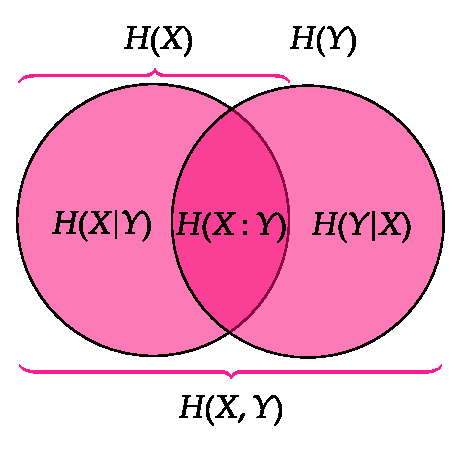
\includegraphics[scale=0.8]{fig/venn-entropy.pdf}
	\caption{Venn diagram showing the relationships between various entropic quantities associated with two random variables.}
\end{figure}